\chapter{Software tester}
\section{G\'{e}n\'{e}ralit\'{e}s sur le test}

Pour répondre à la question \textquote{Qu'est-ce qu'un test?}, je dirais que c'est un code vérifiant le bon fonctionnement d'un code. Il existe de nombreux niveaux de test : unitaire, fonctionnel, d'intégration, de performance, UI, \ldots. Les tests sont très importants dans un projet logiciel, ils permettent de détecter des bugs et de s'assurer du bon fonctionnement du logiciel. La mise en place de ces tests est facilitée par un Framework, il en existe de nombreux mais de manière générale un Framework est un ensemble de librairies et de normes ( de modélisation, d'architecture, ...)\footnote{Source : \url{https://boulaich.wordpress.com/2009/07/08/framework-generalite/}}. \\
\subsection{Description des différents types de test}

%vas voir ici!!! http://jmdoudoux.developpez.com/cours/developpons/java/chap-frameworks-test.php


\subsubsection{Le test unitaire}
Un test unitaire vérifie le bon fonctionnement d'une petite portion de code. En règle générale il ne s'agit que de tester que la valeur retournée par une méthode est la bonne. Mais il s'agit aussi de valider le fonctionnement de la méthode aux limites et de vérifier la cohérence de ses résultats. Ces tests sont censés être les plus nombreux pour couvrir le maximum de cas possibles, on appelle cela le test coverage (ou couverture de test).

\subsubsection{Le test fonctionnel}
Le test fonctionnel est axé sur l'interaction des différentes méthodes. Ces tests permettent de vérifier le bon fonctionnement des spécifications du produit.

\subsubsection{Le test d'intégration}
Le test d'intégration est au test fonctionnel ce que le test fonctionnel est au test unitaire. Le test d'intégration s'assure du bon fonctionnement du logiciel en interaction avec d'autres logiciels.

\subsubsection{Le test de performance}
Le test de performance s'assure qu'une action est effectuée dans le temps imparti. Les actions testées sont aux minimum celles qui composent les workflows nominaux, tant séparément qu'ensemble.

\subsubsection{Le test de stabilité}
Le test de stabilité permet de tester qu'un comportement est systématique, autrement dit qu'une même action implique toujours le même résultat.

\subsubsection{Le test de scalabilité}
Le test de scalabilité permet de s'assurer que le logiciel peut évoluer de manière à pouvoir offrir les mêmes performances dans un contexte d'utilisation qui a évolué. Par exemple, dans le cas où la charge d'utilisation double, est-il possible de modifier l'architecture du logiciel afin que les utilisateurs profitent des mêmes performances?


\subsubsection{Le test de validation de plateforme}
Ce type de test est consacré aux logiciels destinés à être utilisés sur plusieurs plateformes. Est-il possible de l'installer sur plusieurs OS? Les comportements sont-ils les mêmes?

\section{Le test \`{a} SAP}


SAP utilise un grand nombre d'outils pour g\'{e}rer le code de ses produits, poss\'{e}dant chacun plusieurs branches, et pour chacune d'entre elles une suite de tests est ex\'{e}cut\'{e}e quotidiennement. Globalement, les codes, quels qu'ils soient, sont h\'{e}berg\'{e}s sur le gestionnaire de code source Perforce\index{Perforce}. La compilation journali\`{e}re est ex\'{e}cut\'{e}e par Jenkins ou ASTEC, d\'{e}pendamment des \'{e}quipes et des produits, dont les r\'{e}sultats sont automatiquement envoy\'{e}s aux personnes concern\'{e}es (cf. annexe \ref{pdf:automationResults} page \pageref{pdf:automationResults} qui pr\'{e}sente l'un de ces mails automatiques).\\



Les ST\index{Software Tester} sont r\'{e}guli\`{e}rement tenus au fait des tests \`{a} impl\'{e}menter aussi bien par Jira\index{Jira} ou Java Correction WorkBench\index{Java Correction WorkBench} que par liste de distribution de mails (cf. figure \ref{figure:testProcess} page \pageref{figure:testProcess} pour le process complet).\\
\begin{figure}[!ht]
  \centering
      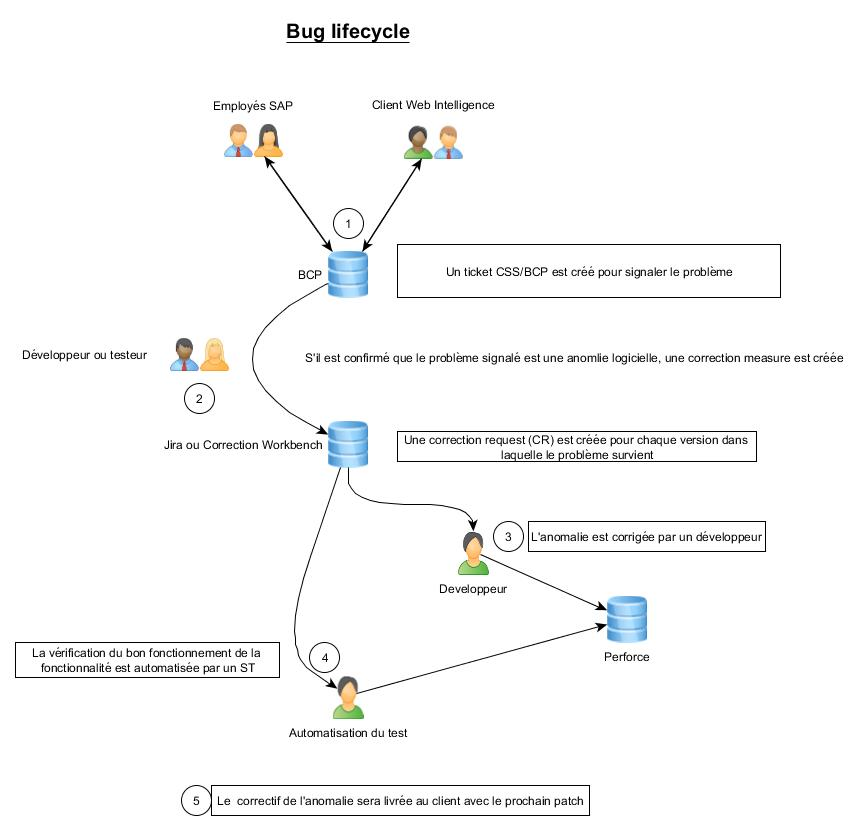
\includegraphics[width=\textwidth]{images/testProcessAtSAP.jpg}
  \caption{Le process de test}
	\label{figure:testProcess}
\end{figure}



\section{Pr\'{e}sentation du produit test\'{e} : WebI}
WebI est un logiciel de BI\index{Business Intelligence} permettant d'acc\'{e}der \`{a} des donn\'{e}es stock\'{e}es en ligne dans un \textquote{univers} (historiquement .unv, maintenant .unx). L'acc\`{e}s aux donn\'{e}es peut se faire via rich client\index{Rich Client} via applet ou via le client dhtml.


\section{Pr\'{e}paration aux tests}






Testeur fût ma premi\`{e}re mission lors de mon arriv\'{e}e \`{a} SAP et je le suis rest\'{e} sur toute la premi\`{e}re p\'{e}riode de mon contrat, c'est-\`{a}-dire 2 mois et demi. Avant de commencer \`{a} impl\'{e}menter des tests, j'ai \'{e}t\'{e} accueilli par mes coll\`{e}gues et on m'a fourni le mat\'{e}riel n\'{e}cessaire au bon d\'{e}roulement de mes missions.\\
Mes 1\up{er} jours \`{a} SAP se sont d\'{e}roul\'{e}s de la mani\`{e}re suivante :\\
\begin{itemize}
\item Pr\'{e}sentation \`{a} l'\'{e}quipe et visite des locaux
\item R\'{e}union avec mon tuteur et mon manager pour une description de la mission
\item R\'{e}cup\'{e}ration des diff\'{e}rents droits d'acc\`{e}s aux serveurs
\item Familiarisation avec les outils internes (tickets HR, CSS, IT, ...)
\item Installation des logiciels n\'{e}cessaires au d\'{e}veloppement (IDE, SCM\index{Source Code Management}, \'{e}diteur de texte, \ldots)
\item Mise en place du framework de test (cr\'{e}ation du workspace perforce) \`{a} l'aide de Christophe DOLIMONT\footnote{voir organigramme de l'équipe \ref{} page \pageref{} }
\end{itemize}
Au terme de la 1\up{\`{e}re} semaine, j'ai pu commencer \`{a} \'{e}tudier le framework de test en me basant sur les tests d\'{e}j\`{a} existants.\\
C'est au cours de la deuxi\`{e}me semaine que j'ai pu impl\'{e}menter mes 1\up{er} tests.

%\glspl{pois} \\
%\glspl{vache} \\
%\glspl{pigeon} \\
% \glspl{TEM}  \\
% \gls{latex}  \\
%\glspl{lvm}



\section{Synth\`{e}se des premières missions}

Tout au long de cette mission, ou plutôt ces missions (un test achev\'{e} laisse toujours la place \`{a} un autre), j'ai travaill\'{e} \`{a} impl\'{e}menter des codes java permettant de tester automatiquement le comportement de WebI au niveau SDK.

L'objectif principal de cette mission \'{e}tait d'\^{e}tre, \`{a} terme, capable d'impl\'{e}menter seul et dans les plus brefs d\'{e}lais un test automatique. La grande difficult\'{e} de d\'{e}but de cette mission a \'{e}t\'{e} de comprendre, d'une part, la logique de test du framework\index{Framework} de test, et d'autre part les diff\'{e}rentes choses que celui-ci me permettait de faire. J'ai distingu\'{e} les quelques points suivants qui sont pour moi l'essentiel qu'un testeur doit maitriser : 
\begin{itemize}
	\item L'int\'{e}gration du test \`{a} la suite de tests 
  \item Quel type de test mettre en place, statique ou dynamique?
	\item Comment initialiser un test, les constructeurs des tests dynamiques peuvent se baser sur un wid\index{wid}, une queryspec\index{queryspec} ou rien du tout
	\item Les tests ne se basant pas sur les m\^{e}mes versions du produits, les JARs\index{JAR}\footnote{Java ARchive : stock les définitions de classes} ne sont jamais les m\^{e}mes
	\item Où trouver les fichiers de références n\'{e}cessaires
	\item Respect absolu des conventions de nommage
\end{itemize}











\subsection{Tests statiques ou dynamiques}

Le test, qu'il soit statique ou dynamique, sera ex\'{e}cut\'{e} avec tous les autres d\`{e}s lors que le nom du test plan est inscrit dans la test suite\index{Testsuite}.\\
La diff\'{e}rence fonctionnelle entre ces deux types de tests est que l'un ne fait que comparer deux documents WebI alors que l'autre permet d'appliquer un certain nombre des modifications sans pour autant les comparer syst\'{e}matique \`{a} la fin.\\
La diff\'{e}rence en terme de consommation de temps est tr\`{e}s importante, puisque pour un test statique il n'est pas n\'{e}cessaire d'impl\'{e}menter de testcase\index{Testcase}! Il suffit de g\'{e}n\'{e}rer la r\'{e}f\'{e}rence, de la mettre dans le dossier d\'{e}di\'{e}, compl\'{e}ter le script.xml et la test suite, impl\'{e}menter le test plan et finalement livrer le code impl\'{e}menté. Voyons ceci plus en d\'{e}tail.

\subsubsection{Tests statiques}
Globalement, le test statique :

\begin{itemize}
	\item ne fait que comparer un document par rapport \`{a} une r\'{e}f\'{e}rence
	\item ne demande que tr\`{e}s peu de connaissances techniques, que ce soit en Java ou sur WebI
\end{itemize}

\textbf{Principe du test statique}\hfill \\ \indent
Lors de l'ex\'{e}cution d'un test statique, un fichier est g\'{e}n\'{e}r\'{e} \`{a} partir d'un wid\index{wid}. Le format du fichier ainsi g\'{e}n\'{e}r\'{e} (txt\_\footnote{type personnalis\'{e} interne \`{a} SAP}, txt ou doc) est pr\'{e}cis\'{e} dans le fichier script.xml.\\
Ensuite, \`{a} la fin de l'ex\'{e}cution du test, ce fichier g\'{e}n\'{e}r\'{e} est compar\'{e} \`{a} un fichier de r\'{e}f\'{e}rence.\\
Si les deux fichiers sont identiques, le test est correct, sinon il \'{e}choue.\\
Pour l'ex\'{e}cution d'un test statique, il ne faut qu'impl\'{e}menter un testplan qui respecte la structure suivante :

\lstinputlisting[language=java]{scripts/basicStaticTest.java}

Une fois ceci fait il est n\'{e}cessaire de g\'{e}n\'{e}rer le fichier de r\'{e}f\'{e}rence. Cela se fait en ex\'{e}cutant le test une 1\up{\`{e}re} fois en mettant l'option savingtxt\footnote{Pour g\'{e}n\'{e}rer une resource .txt, savingdoc pour g\'{e}n\'{e}rer un doc, etc.} du script.xml \`{a} true (voir figure \ref{figure:scriptXmlSavingRef} page \pageref{figure:scriptXmlSavingRef})

\begin{figure}[!ht]
  \centering
      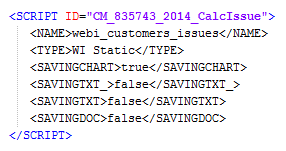
\includegraphics{images/scriptXmlSavingRef.png}
  \caption{Contenu du script.xml pour g\'{e}n\'{e}rer une r\'{e}f\'{e}rence}
	\label{figure:scriptXmlSavingRef}
\end{figure}

\`{A} cette \'{e}tape, l'ex\'{e}cution du test \'{e}chouera puisqu'il n'y a pas de r\'{e}f\'{e}rence.\\
Le fichier de r\'{e}f\'{e}rence ainsi g\'{e}n\'{e}r\'{e} doit \^{e}tre copié depuis le r\'{e}pertoire de r\'{e}sultat puis coll\'{e} dans le dossier où sont stock\'{e}s les fichiers de ressources (voir la figure \ref{figure:testEmptyShell} page \pageref{figure:testEmptyShell} pour avoir une illustration des diff\'{e}rents fichiers et dossiers dans l'architecture du framework de test).







\subsubsection{Tests dynamiques}

\`{A} la diff\'{e}rence du test statique, le test dynamique va modifier le document apr\`{e}s ouverture. Ceci permettant de s'assurer que la m\'{e}canique interne de WebI produit l'effet escompt\'{e} sur le document. La comparaison avec un document de r\'{e}f\'{e}rence est bien \'{e}videmment possible mais pas syst\'{e}matique, il suffit souvent de tester la valeur ou l'existence d'un objet.\\
D'un point de vue g\'{e}n\'{e}ral, un testplan respecte l'impl\'{e}mentation suivante :


\lstinputlisting[language=java,label=basicDynamicTestPlan]{scripts/basicDynamicTestPlan.java}


Et son testcase respecte l'impl\'{e}mentation suivante :

\lstinputlisting[language=java,label=basicDynamicTestCase]{scripts/basicDynamicTestCase.java}

\`{A} la lecture du test case, on peut observer le constructeur de la super classe, celui-ci prends un certain nombre d'arguments. Il existe dix constructeurs diff\'{e}rents pour la super classe MonoDocTestCase mais deux sont particuli\`{e}rement important. L'un permet de baser son test sur un document g\'{e}n\'{e}r\'{e} \`{a} partir d'une queryspec\index{queryspec}, l'autre sur un document .wid\index{wid}. Par exemple le constructeur se basant sur un wid\index{wid} :\\
\begin{lstlisting}
MonoDocTestCase(MonoDocTestCaseConfigInfo tccInfo, String sDocumentName, String sCategoryType, String sCategory, Boolean useAuroraCtx);
\end{lstlisting}
où
\begin{description}
	\item[tccInfo] \hfill \\
	Objet contenant les informations g\'{e}n\'{e}rales relatives au test case
	\item[sDocumentName] \hfill \\
	Nom du document .wid\index{wid} qui sera charg\'{e} lors de la construction de l'objet
	\item[sCategoryType] \hfill \\
	Nom de la cat\'{e}gorie, en g\'{e}n\'{e}ral : \textquote{corporate}
	\item[sCategory] \hfill \\
	Path du dossier dans lequel est stock\'{e} le .wid\index{wid}. Doit respecter la nomenclature suivante : /auto/\{scriptname\}/wid\index{wid}
	\item[useAuroraCtx] \hfill \\
	Le test en question porte t-il sur aurora?
\end{description}
 Dans tous les cas, lorsque l'objet testcase est instanci\'{e}, nous pouvons impl\'{e}menter un code manipulant le document au niveau SDK\index{SDK}, ce qui signifie que l'on ne simule pas un clic sur un bouton mais que l'on appelle l'une des m\'{e}thodes \textquote{derri\`{e}re} ce bouton, reproduisant ainsi le comportement au niveau SDK d'une manipulation au niveau GUI\index{Graphical User Interface}\footnote{Graphical User Interface}







\subsubsection{Ex\'{e}cution d'un test}


Lors de l'ex\'{e}cution d'un test, plusieurs fichiers sont g\'{e}n\'{e}r\'{e}s en divers endroits. Il y a par exemple :
\begin{description}
\item[Les fichiers de log] \hfill \\ Ces fichiers contiennent des information telles que les exceptions levées ou tout autre informations que va générer le logger
\item[La sortie console] \hfill \\
Enregistr\'{e}e dans \\ \ldots\textbackslash{}Workspace\_Aurora\textbackslash{}rebean\textbackslash{}logs\textbackslash{}\{scriptname\}
\item[Les fichiers g\'{e}n\'{e}r\'{e}s] \hfill \\
Enregistr\'{e}s dans \begin{sloppypar} \ldots\textbackslash{}Workspace\_Aurora\textbackslash{}rebean\textbackslash{}results\textbackslash{}Your Build Number\textbackslash{}res\textbackslash{}\{ scriptName\}\textbackslash{}CM\_\{cmNumber\}\_\{short text\}\textbackslash{}\end{sloppypar}uniquement si l'enregistrement des ressources est sp\'{e}cifi\'{e} dans le script.xml\\
Si savingDoc est \`{a} True, le document de r\'{e}f\'{e}rence est enregistr\'{e} sur le CMS\index{CMS} dans le dossier Folders/Public Folders/auto/, voir l'illustration \ref{figure:savedReferenceDocPath} page \pageref{figure:savedReferenceDocPath}, et le document g\'{e}n\'{e}r\'{e} est enregistr\'{e} dans My Documents/My Favorites/Personnals Documents, voir l'illustration \ref{figure:savedGeneratedDocPath} page \pageref{figure:savedGeneratedDocPath}
\begin{figure}[H]
  \centering
      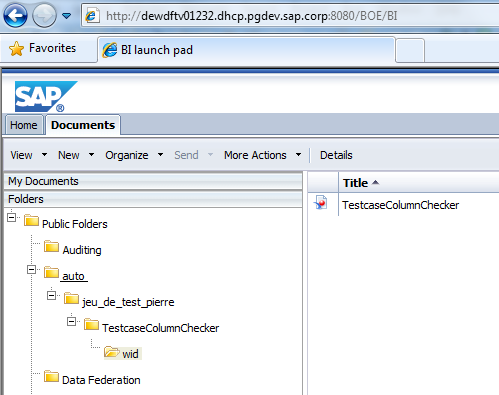
\includegraphics{images/savedReferenceDocPath.png}
  \caption{Capture d'\'{e}cran de WebI de l'arborescence du document de r\'{e}f\'{e}rence}
	\label{figure:savedReferenceDocPath}
\end{figure}
\begin{figure}[H]
  \centering
      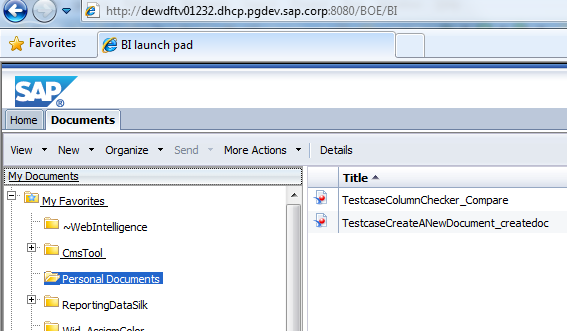
\includegraphics{images/savedGeneratedDocPath.png}
  \caption{Capture d'\'{e}cran de WebI de l'arborescence du document g\'{e}n\'{e}r\'{e}}
	\label{figure:savedGeneratedDocPath}
\end{figure}


\item[Les fichiers ressources] \hfill \\
Les .wid\index{wid} sont enregistr\'{e}s en local dans le répertoire \\ \ldots\textbackslash{}Resources\_AURORA\textbackslash{}storage\textbackslash{}auto\textbackslash{}\{ scriptName\}\textbackslash{}wid\index{wid}\\
et les autres documents de r\'{e}f\'{e}rences (txt, html, etc.) sont dans \\ \ldots\textbackslash{}Resources\_AURORA\textbackslash{}storage\textbackslash{}auto\textbackslash{}\{scriptName\}\textbackslash{}CM\_\{cmNumber\}\_\{short text\}\textbackslash{}\\ 
voir une illustration de cette arborescence figure \ref{figure:localSavedReferences} page \pageref{figure:localSavedReferences}
\begin{figure}[!ht]
  \centering
      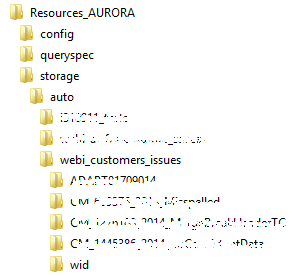
\includegraphics{images/localSavedReferences.png}
  \caption{Capture d'\'{e}cran de WebI de l'arborescence des r\'{e}f\'{e}rences locales}
	\label{figure:localSavedReferences}
\end{figure}
\item[Les logs du serveur tomcat] \hfill \\
Disponible dans le dossier d'installation du serveur ces logs sont trop verbeux pour pouvoir \^{e}tre utilisés systématiquement. Mais ils restent une précieuse source d'informations et sont utiles dans certains cas.
\end{description}





\subsection{De l'\'{e}tude \`{a} l'int\'{e}gration}

D'abord, les demandes de tests automatiques ne sont pas toujours r\'{e}alisables au niveau SDK. Il convient donc de v\'{e}rifier, en 1\up{er} lieu, la faisabilit\'{e} du test. Une fois que l'on sait que la r\'{e}alisation est possible et que l'on a choisi une strat\'{e}gie de test, il faut pr\'{e}parer l'environnement de travail, c'est-\`{a}-dire construire la coquille vide du test d\'{e}sir\'{e}.


\subsubsection{Analyse du test \`{a} impl\'{e}menter}
\begin{description}
	\item[\'{E}tudier le bug] Au pr\'{e}alable, toutes les informations que l'on a sur le bug \`{a} tester se trouvent sur JCWB\index{Java Correction WorkBench} (voir figure \ref{figure:JCWB-CRs} page \pageref{figure:JCWB-CRs}), les informations nous concernant sont :
\begin{itemize}
	\item L'identifiant du defect (utilisé par les conventions de nommage)
	\item La description détaillée du bug
	\item Le workflow provoquant le bug
	\item La/Les branche(s) sur laquelle/lesquelles il a été décelé
\end{itemize}

	\begin{figure}[!ht]
  \centering
      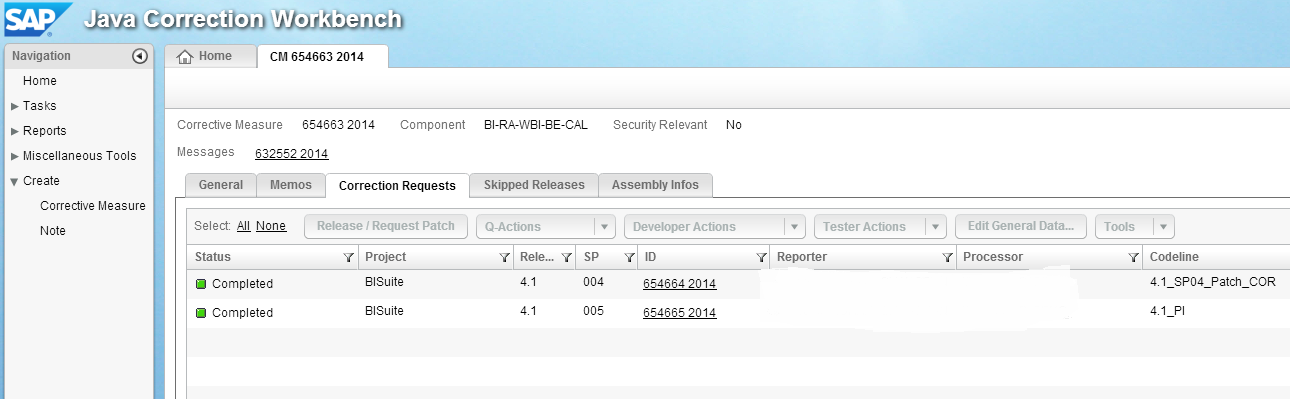
\includegraphics[width=\textwidth]{images/JCWB-CRs.png}
  \caption{\'{E}cran de JCWB propre \`{a} une CM\index{Correction Measure}}
	\label{figure:JCWB-CRs}
\end{figure}
Ceci fait, il est int\'{e}ressant d'aller \'{e}tudier le code qui a \'{e}t\'{e} modifi\'{e} pour corriger le bug. Cela permet de se faire une idée des objets provoquant le bug ainsi que les méthodes corrigées dont il faut maintenant tester le bon fonctionnement. Pour cela il suffit d'aller dans Perforce et de rechercher la modification effectuée. Un clic droit sur la changelist en question offre la possibilité d'utiliser la fonction \textquote{diff against previous revision} du SCM\index{Source Code Management} pour obtenir la liste exhaustive des fichiers modifi\'{e}s ainsi qu'un vis-\`{a}-vis entre les versions pr\'{e}-correctif et post-correctif (voir figure \ref{figure:diffAgainst} page \pageref{figure:diffAgainst})\\
	\begin{figure}[!ht]
  \centering
      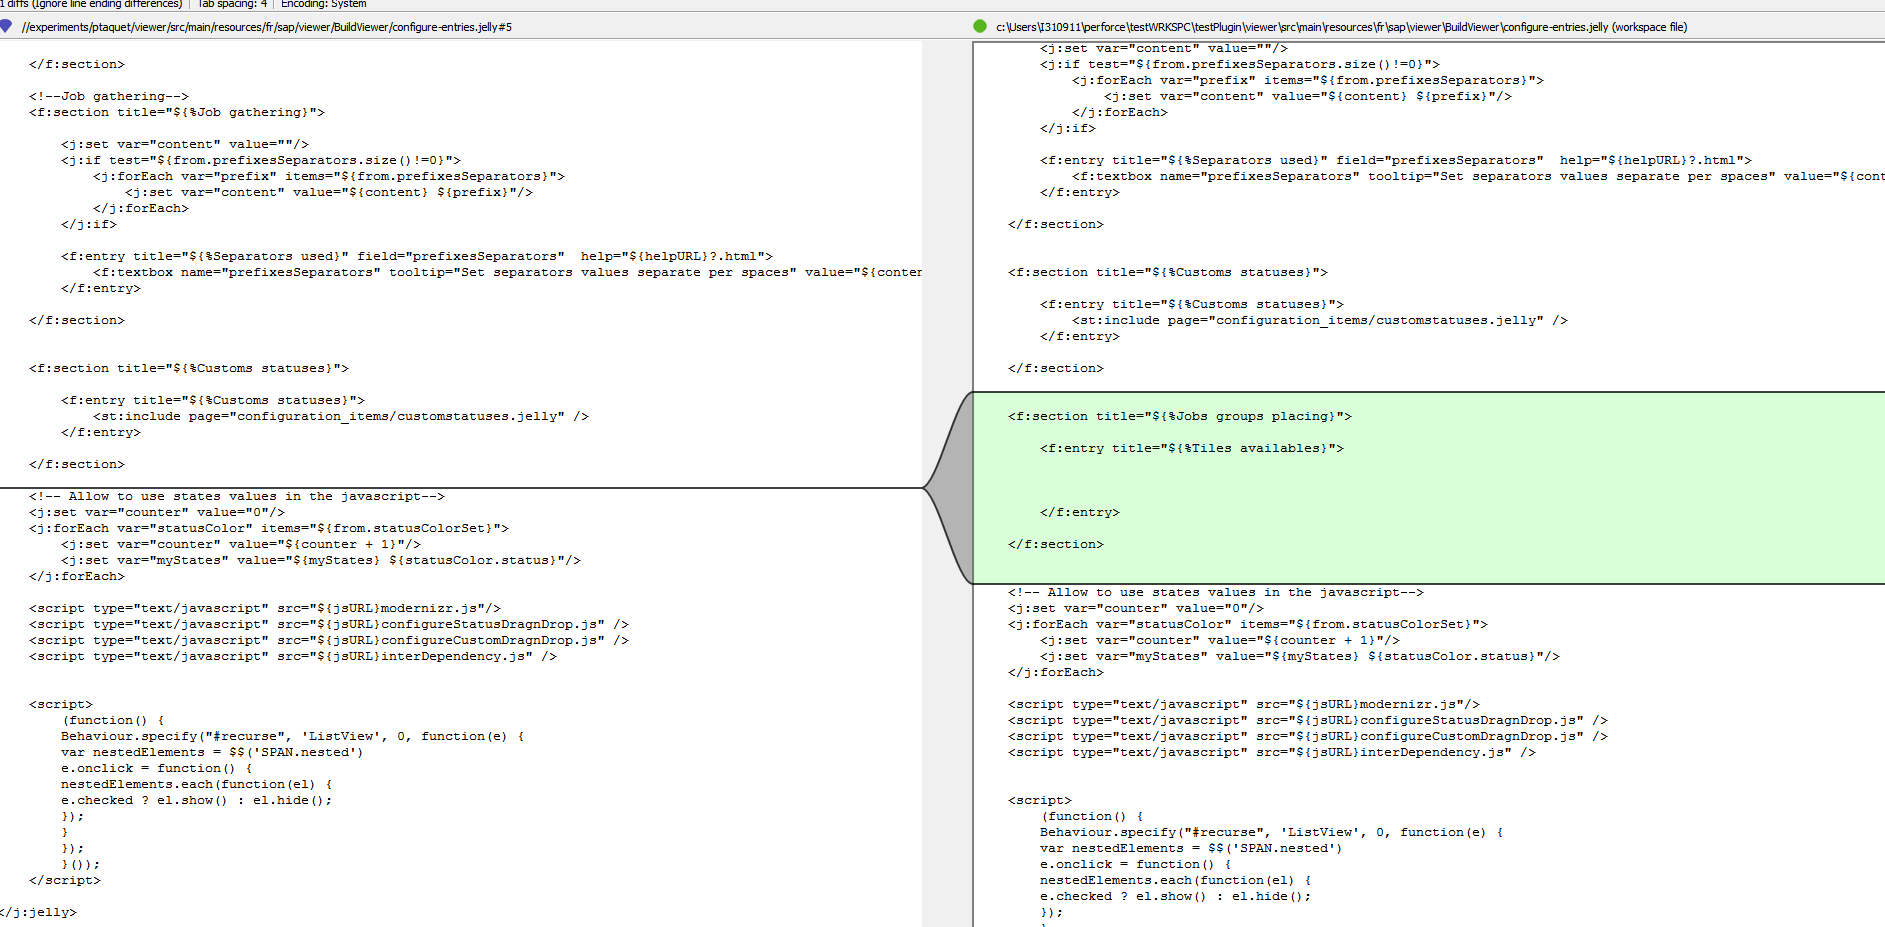
\includegraphics[width=\textwidth]{images/diffAgainst.png}
  \caption{\'{E}cran de comparaison des 2 versions d'un m\^{e}me fichier (avant et apr\`{e}s correctif)}
	\label{figure:diffAgainst}
\end{figure}

	\item[Reproduire le probl\`{e}me] Une fois que le bug est compris, il nous incombe de reproduire \`{a} la main le workflow et de valider l'existence du bug sur la version bugg\'{e}e ainsi que le bon fonctionnement de la version corrig\'{e}e. \`{A} cette \'{e}tape, si le bug survient sur le CMS\index{CMS} (client l\'{e}ger), il est int\'{e}ressant d'utiliser le debugger du navigateur pour observer les donn\'{e}es transitant.
	
	\item[D\'{e}finir la strat\'{e}gie de test] Maintenant que le probl\`{e}me est bien compris et localis\'{e}, nous pouvons savoir s'il est possible de le tester. Si non, soit le probl\`{e}me ne peut pas \^{e}tre test\'{e} soit nous redirigeons la correction vers l'\'{e}quipe de testeurs concern\'{e}e (plus ou moins haut ou bas niveau).\\
Si l'impl\'{e}mentation du test est possible, il faut choisir la meilleure mani\`{e}re de tester l'existence et la non-existence du bug ainsi que le moyen le plus rapide d'arriver \`{a} reproduire le probl\`{e}me. Par exemple, faut-il un test statique ou dynamique? Partir d'une queryspec\index{queryspec} ou d'un document .wid\index{wid}?
\end{description}


\subsubsection{Impl\'{e}mentation de la coquille vide}
L'int\'{e}r\^{e}t de coder d'abord la coquille vide est d'avoir un code qui compile mais qui ne fait encore rien. Ce qui garantit que tout a bien été nommé, test case et script.xml. Et, en fonction du besoin, s'assurer de la g\'{e}n\'{e}ration sur le serveur des .wid\index{wid}.\\ 
Comme sch\'{e}matis\'{e} figure \ref{figure:testsRelations} page \pageref{figure:testsRelations}, chaque test automatique est int\'{e}gr\'{e} \`{a} un test plan, lui-m\^{e}me \'{e}tant int\'{e}gr\'{e} \`{a} une test suite.\\
\begin{figure}[!ht]
  \centering
      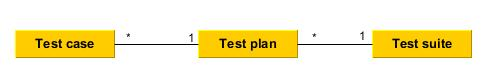
\includegraphics[width=\textwidth]{images/testsRelations.jpg}
  \caption{Diagramme UML des suites de tests}
	\label{figure:testsRelations}
\end{figure}

Ci-dessous les fichiers \`{a} impl\'{e}menter :\\
\begin{enumerate}
	\item \textbf{Test plan} Cr\'{e}er le nouveau test plan dans le package correspondant au client qui a remont\'{e} le bug (dans testplans.rebean\_wi.customers.\{clientID\}). Renseigner toutes les informations relatives au test, si ce fichier est correctement impl\'{e}ment\'{e} il ne sera plus n\'{e}cessaire de le modifier par la suite. Voir l'implémentation d'exemple partie \ref{basicDynamicTestPlan} page \pageref{basicDynamicTestPlan}).
	\item \textbf{Test case} Uniquement dans le cas du test dynamique. Cr\'{e}er le test case dans le package correspondant au client (dans testcases.aurora\_customers.\{clientID\}). Attention \`{a} respecter le pattern de nommage \textquote{CM\_\{CM\_id\}\_shortText}, voir l'implémentation d'exemple partie \ref{basicDynamicTestCase} page \pageref{basicDynamicTestCase}.
	\item \textbf{Test suite} Dans le package des tests plan, on peut trouver la test suite qu'il faut modifier. Il suffit de rajouter le nom du test plan \`{a} la liste de test plan que la test suite ex\'{e}cute.
	\item \textbf{script.xml} Ajouter les diff\'{e}rents param\`{e}tres correspondants au test.
	\item \textbf{ressources} G\'{e}n\'{e}rer les documents ressources n\'{e}cessaires (queryspec\index{queryspec}, .wid\index{wid}, etc.) et les ajouter au dossier portant le nom de la CM\index{Correction Measure} (respect de la convention de nommage), garantissant l'unicité de ce dossier.
	\item \textbf{parameters.xml} Renseigner l'url du CMS\index{CMS} cibl\'{e} et mettre \`{a} jour les extracted JARs permettant la compilation du test vide
	\item V\'{e}rifier que tous les éléments nécessaires sont dans la change list de perforce, puis \textquote{push} les modifications.
\end{enumerate}


D'une mani\`{e}re g\'{e}n\'{e}rale, la structure \`{a} connaitre pour impl\'{e}menter correctement la coquille vide est illustr\'{e}e figure \ref{figure:testEmptyShell} page \pageref{figure:testEmptyShell}. L'utilisation de ces fichiers ou dossiers est sytématique pour certains et quasi-systématique pour d'autres, les connaître est essentiel. Et, comme illustré figure \ref{figure:usedFilesForTests} page \pageref{figure:usedFilesForTests}, il est important de savoir à partir de quoi l'on peut construire un test et ce qu'il est possible de générer par celui-ci.\\
\begin{figure}[H]
  \centering
      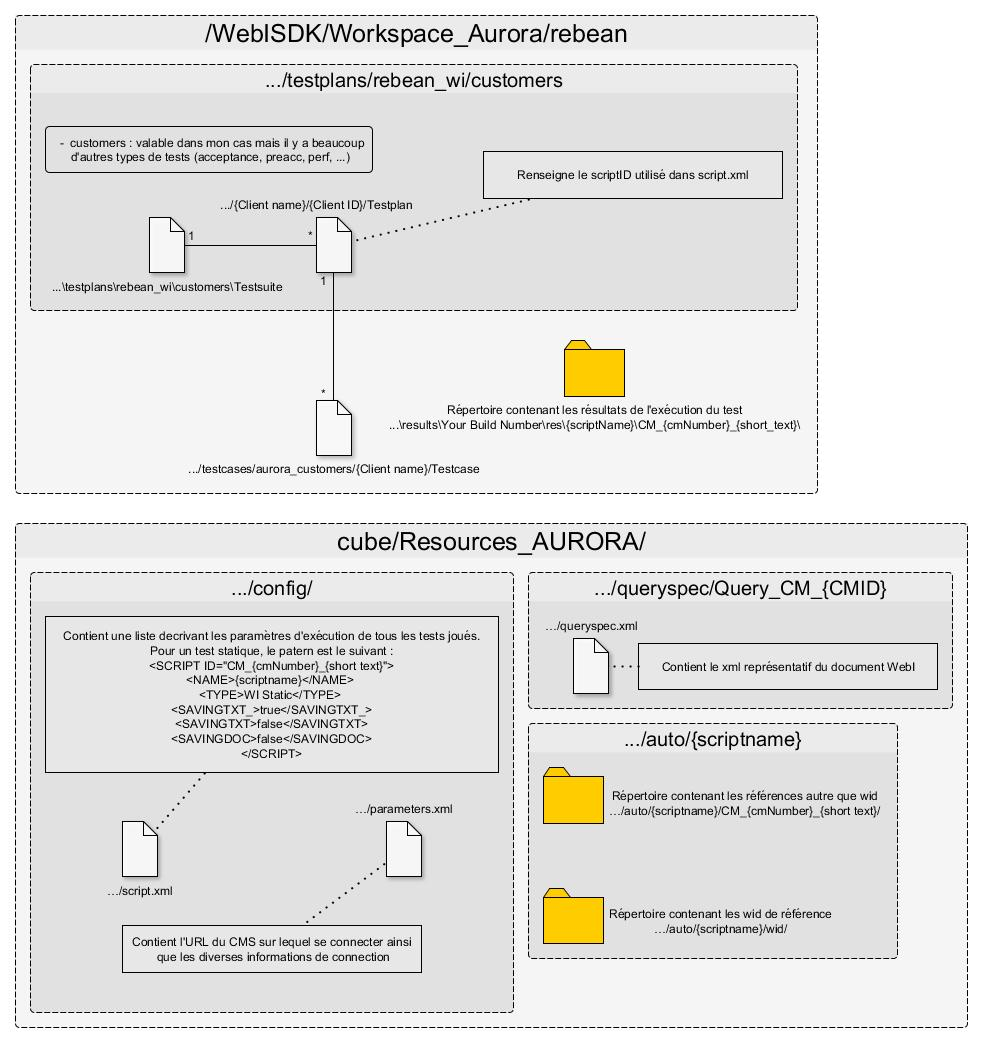
\includegraphics[width=\textwidth]{images/testEmptyShell.jpg}
  \caption{Diagramme repr\'{e}sentant les diff\'{e}rents \'{e}l\'{e}ments qui compose la coquille vide d'un test dynamique}
	\label{figure:testEmptyShell}
\end{figure}
\begin{figure}[H]
  \centering
      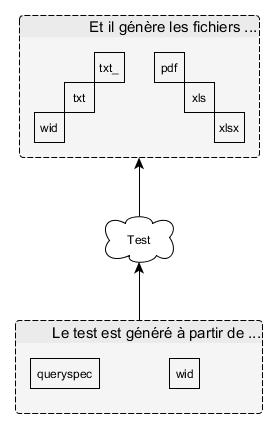
\includegraphics[width=0.4\textwidth]{images/usedFilesForTests.jpg}
  \caption{Les fichiers utilisés ou générés par le test}
	\label{figure:usedFilesForTests}
\end{figure}

\subsubsection{Les ressources}
Les ressources sont tr\`{e}s importantes dans le contexte du test, celles-ci se pr\'{e}sentent sous plusieurs jours diff\'{e}rents :
\begin{enumerate}
	\item un document .wid\index{wid} cr\'{e}é en suivant \`{a} la lettre le workflow \`{a} tester mais dont la construction a \'{e}t\'{e} arr\^{e}t\'{e}e juste avant que ne survienne le bug.\\
	Cette ressource sert \`{a} utiliser un document d\'{e}j\`{a} construit et permet au ST\index{Software Tester} de n'automatiser que la partie \`{a} tester.
	\item un fichier (txt, txt\_, pdf, doc, xls, xls, ...) consid\'{e}r\'{e} comme une r\'{e}f\'{e}rence\\
	Cette ressource est compar\'{e}e au document obtenu \`{a} la fin du workflow pour garantir la similitude.\\
	Cette ressource est générée à l'exécution du test à partir du document en cours, il faut donc d'abord le copier/coller depuis le répertoire où est générée cette ressource vers celui où la référence sera récupérée.\\
	Une question se pose alors : cette référence que j'ai ainsi généré est-elle garantie sans erreur?
	\item une queryspec\index{queryspec}, c'est un fichier xml repr\'{e}sentatif du document .wid\index{wid}
\end{enumerate}

\textbf{Obtenir un fichier wid\index{wid}}
\begin{description}
	\item	[Via le CMS\index{CMS}] 
	\begin{sloppypar}
	Il suffit de parcourir l'arborescence du CMS\index{CMS} pour arriver \`{a} l'emplacement du .wid\index{wid}. Dans les propi\'{e}t\'{e}s du fichier, il y a son nom complet (diff\'{e}rent du nom dans WebI) avec son arborescence \`{a} partir du dossier Input (figure \ref{figure:widFileLocation} page \pageref{figure:widFileLocation} ). Ensuite, dans le syst\`{e}me de fichiers du serveur (par exemple : \textquote{\textbackslash{}\textbackslash{}dewdftv01634.dhcp.pgdev.sap.corp\textbackslash{}c\$}) aller dans 
	\textquote{\textbackslash{}Program Files (x86)\textbackslash{}SAP BusinessObjects\textbackslash{}SAP BusinessObjects Enterprise XI 4.0\textbackslash{}FileStore\textbackslash{}Input} et copier/coller le chemin d'acc\`{e}s au fichier. Le document .wid\index{wid} se trouve dans le r\'{e}pertoire en question.
	\end{sloppypar}
\begin{figure}[!ht]
  \centering
      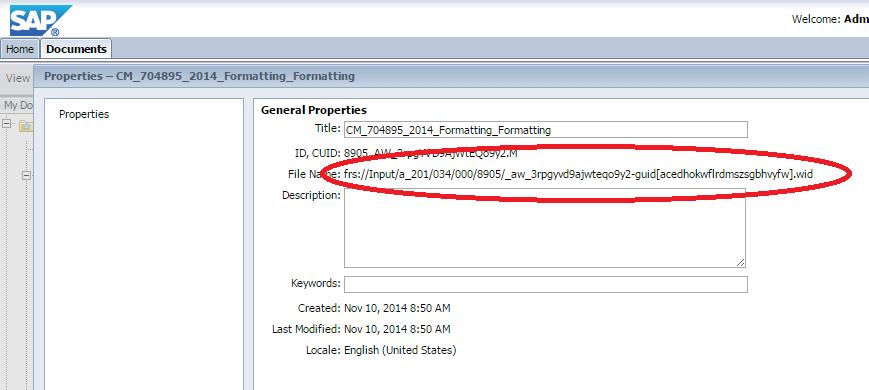
\includegraphics[width=\textwidth]{images/widFileLocation.png}
  \caption{Capture de l'\'{e}cran de propri\'{e}t\'{e} d'un document WebI}
	\label{figure:widFileLocation}
\end{figure}
	\item[Via le Rich Client]
	Attention \`{a} la version du rich client qui doit \^{e}tre la m\^{e}me que celle du CMS\index{CMS}. Ouvrir une connexion point\'{e}e sur le bon CMS\index{CMS}, ouvrir le document d\'{e}sir\'{e} et enregistrer sous le document .wid\index{wid}.
\end{description}

\clearpage
\section{Bilan de la 1\up{ère} période}
Tout au long des mois de juillet, ao\^{u}t et septembre j'ai impl\'{e}menté de nombreux tests\footnote{cf. annexe \ref{pdf:ImplementedTestsList} page \pageref{pdf:ImplementedTestsList} pour la liste compl\`{e}te des tests impl\'{e}ment\'{e}s} pour des bugs divers, que ce soit une faute de frappe ou une fonctionnalité ne fonctionnant plus du tout. J'ai beaucoup appris de mes erreurs, surtout lorsque plusieurs jours de travail s'av\'{e}raient inutiles parce qu'une meilleure solution, \'{e}vidente pour qui sait, existait.\\
J'ai aussi pu parfaire mes connaissances en Java ainsi que ma méthodologie lorsque je dois me former à une nouvelle technologie.\\
Au début de cette mission, je n'avais jamais implémenté de tests à l'exception de tests unitaires. Aujourd'hui, je suis ravi de comprendre la problématique du test et quels types de tests existent. Aujourd'hui je sais pourquoi et comment les implémenter et suis capable de faire des tests qui soient facilement maintenables.



\subsection{Connaissance du framework}
La principale perte de temps était dûe à une méconnaissance du Framework de test. Celui-ci possédant un grand nombre de méthodes aux intérêts divers et variés, d'emblée, il est très difficile de pouvoir déterminer laquelle utiliser. D'autant plus qu'au moment où le besoin de telle ou telle méthode se faisait sentir, je n'avais pas connaissance de son existence. En conséquence, je me suis vu trop souvent implémenter des méthodes déjà existantes, me faisant perdre un temps précieux.\\
L'expérience accumulée durant cette période m'a permis de ne plus perdre de temps à ré-inventer la roue et de me concentrer sur le code ad hoc nécessaire à un test précis et fiable.

\subsection{Méthodologie}
L'autre grande perte de temps venait surtout de ma méconnaissance du produit testé. Certaines fonctionnalités étant très complexes il m'arrivait de ne pas identifier exactement le problème pour finalement perdre du temps à implémenter du code inefficient.\\
Le meilleur exemple que je puisse citer s'est produit quand j'ai commencé à tester des bugs intégrés à des workflows complexes. Un certain nombre de manipulations et/ou de configurations était alors nécessaire pour que le bug survienne. Et c'est dans ces conditions que j'ai implémenté la quasi totalité du workflow au niveau SDK pour finalement arriver sur la zone à tester. Le test fonctionnait bien, il échouait sur les versions buggées et passait sur les versions fixées. Le problème ne vient pas du test que j'ai implémenté, car celui-ci faisait ce qu'il fallait, mais de la manière. J'ai implémenté ce code en approximativement 3 jours. Alors que si j'avais utilisé le CMS pour générer un document à une étape seulement du bug, et que si j'avais implémenté uniquement l'appel à tester, j'aurais pu implémenter ce test en quelques heures seulement!

\subsection{Travail en équipe}
Le framework de test est entretenu quotidiennement par des dizaines de testeurs implémentant des tests et modifiant le framework lui-même. Le résultat de l'exécution des suites de tests est visible par testeurs, développeurs et par d'autres. J'étais donc intégré à une grande équipe, leurs travaux ayant des répercussion sur les miens, et les miens sur les leurs. Il faut donc faire attention au code que l'on \textquote{push} sur Perforce! L'anecdote me venant à l'esprit s'est passée un vendredi soir, alors que je venais de terminer un test et que celui-ci se comportait bien. J'ai livré mon test sur perforce. L'ennui était que j'utilisais un package dans lequel je mettais des méthodes de test pour ne pas polluer mon test \textquote{final}. Je n'ai malheureusement pas pensé à revoir l'import de mes sources. Mon code, compilant correctement en local, ne compilait plus sur le serveur et a donc fait crashé toute la suite de test. Le mail automatique envoyé à informé tout le monde de mon erreur de manipulation (illustrée annexe \ref{annexe:crashedBuildBecauseOfMe} page \ref{annexe:crashedBuildBecauseOfMe})!\\

J'ai eu aussi la chance de travailler dans une équipe maitrisant très bien le framework et le produit. J'ai appris énormément pendant les entretiens que j'ai eu avec ces différentes personnes.

